\documentclass{article}
\setlength{\parindent}{0ex}
\setlength{\parskip}{1em}
\usepackage[utf8]{inputenc} 
\usepackage{amsfonts}
\usepackage{amssymb}
\usepackage{amsmath}
\usepackage{amstext}
\usepackage{fancybox}
\usepackage{tikz}
\usepackage{tkz-euclide}
\usepackage{gensymb}
\usepackage{graphicx}
\usepackage{verbatim}
\usepackage{qtree}
\usepackage{scrextend}
\usepackage{multirow}
\usepackage{float}

\tikzset{main node/.style={circle,fill=blue!20,draw,minimum size=1cm,inner sep=0pt},
}

%Kodestyling \begin{lstlisting}
\usepackage{color}
\usepackage{listings}
\lstset{ %
language=C++,                % choose the language of the code
%basicstyle=\footnotesize,       % the size of the fonts that are used for the code
basicstyle=\ttfamily,
%numbers=left,                   % where to put the line-numbers
numberstyle=\footnotesize,      % the size of the fonts that are used for the line-numbers
stepnumber=1,                   % the step between two line-numbers. If it is 1 each line will be numbered
numbersep=5pt,                  % how far the line-numbers are from the code
backgroundcolor=\color{white},  % choose the background color. You must add \usepackage{color}
showspaces=false,               % show spaces adding particular underscores
showstringspaces=false,         % underline spaces within strings
showtabs=false,                 % show tabs within strings adding particular underscores
%frame=single,           % adds a frame around the code
tabsize=2,          % sets default tabsize to 2 spaces
captionpos=b,           % sets the caption-position to bottom
breaklines=true,        % sets automatic line breaking
breakatwhitespace=false,    % sets if automatic breaks should only happen at whitespace
escapeinside={\%*}{*)},          % if you want to add a comment within your code
mathescape
}

\usepackage{mathtools}
\DeclarePairedDelimiter\ceil{\lceil}{\rceil}
\DeclarePairedDelimiter\floor{\lfloor}{\rfloor}


\def\meta#1{\mbox{$\langle\hbox{#1}\rangle$}}
\def\macrowitharg#1#2{{\tt\string#1\bra\meta{#2}\ket}}

{\escapechar-1 \xdef\bra{\string\{}\xdef\ket{\string\}}}

\def\intro#1{{#1}{\cal I}}
\def\elim#1{{#1}{\cal E}}

\showboxbreadth 999
\showboxdepth 999
\tracingoutput 1


\let\imp\to
\def\elim#1{{{#1}{\cal E}}}
\def\intro#1{{{#1}{\cal I}}}
\def\lt{<}
\def\eqdef{=}
\def\eps{\mathrel{\epsilon}}
\def\biimplies{\leftrightarrow}
\def\flt#1{\mathrel{{#1}^\flat}}
\def\setof#1{{\left\{{#1}\right\}}}
\let\implies\to
\def\KK{{\mathsf K}}
\let\squashmuskip\relax

\graphicspath{ {images/} }
\usetikzlibrary{arrows}
\tikzset{
  leaf_/.style = {shape=rectangle,draw, align=center},
  node_/.style     = {shape=circle,draw,align=center}
}
\author{Rune Kok Nielsen (qkd362), Andreas Holm (jnh508)}
\title{Afløsningsopgave i fagområdet Modellering og Analyse af Data}
\DeclareMathOperator{\Ran}{Ran}
\DeclareMathOperator{\Dom}{Dom}
\begin{document}

\maketitle

\section{Klassificering}
Formålet med klassificering er at putte datapunkter bestående af et antal egenskaber i passende kategorier fra en prædifineret mængde af diskrete, beskrivende kategorier. Disse datapunkter er også kendt som tupler bestående af $(x,y)$, hvor $x$ er de givne egenskaber, og $y$ er punktets kategori. Klassificering består i definitionen af at finde en passende klassificeringsmodel, hvilket er en funktion $f$ der tager et datapunkt $x$ og returnerer den tilhørende kategori $y$.

Der findes adskillige teknikker til at bestemme en klassificeringsmodel. En sådan teknik beskriver en læringsalgoritme, der på basis af et træningssæt (et sæt af datapunkter med kendte kategorier) udleder en (evt. suboptimal) model.

Det er sjældent muligt at klassificere ethvert givent punkt korrekt ud fra de tilgængelige egenskaber, og vi har derfor brug for en måde at afgøre nøjagtigheden af den resulterende model. Denne nøjagtighed estimeres ved at klassificere et testsæt med modellen, og se på hvor stor en andel af datapunkterne der har fået den rigtige kategori. For at vise modellens nøjagtighed kan man beregne dens \textit{accuracy}, hvilket fortæller hvor præcis den er, eller man kan beregne dens \textit{error rate}, hvilke er det modsatte af \textit{accuracy} dvs. hvor mange forkerte punkter modellen har produceret.\\
For at beregne nøjagtigheden af en model, benytter vi et testsæt. Ligesom træningssættet er testsættet en mængde af datapunkter med kendte kategorier. Udregningerne består da i at klassificere punkterne i testsættet ved hjælp af modellen, og sammenligne punkternes kategorier som udregnet af modellen med deres egentlige kategorier, som vi kender i forvejen.\\
Det er essentielt at testsættet ikke overlapper med træningssættet, da dette vil tildele en for høj nøjagtighed til modellen. Har man f.eks. et meget lille træningssæt kan man nemt lave en model, som tilfældigvis passer perfekt på træningssættet, men som i realiteten er helt forkert. Tester man modellen på et testsæt som næsten overlapper fuldstændigt med træningssættet vil de overlappende punkter højst sandsynligt klassificeres korrekt, hvilket resulterer i meget høj nøjagtighed, selvom modellen i virkeligheden kun passer netop på træningssættet. 

For at beregne nøjagtiheden og fejlraten bruger vi en \textit{confusion matrix}. I bel 1 ses en \textit{confusion matrix}, det ses i kolonnerne hvad modellen har tildelt klassen, og i rækkerne ses hvad dens rigtige klasser er. \\

\begin{table}[H]
\begin{center}
\begin{tabular}{cc|c|c|c|c|}
    & \multicolumn{5}{c}{Predicted Class} \\
    \cline{3-6}
     & & Class = 0 & Class = 1 & .. & Class = n \\
    \cline{2-6}
    \multicolumn{1}{c|}{\multirow{4}{*}{Actual Class}} & Class = 0 & $f_{00}$ & $f_{01}$ & .. & $f_{0n}$ \\
    \cline{2-6}
    \multicolumn{1}{c|}{} & Class = 1 & $f_{10}$ & $f_{11}$ & .. & $f_{1n}$ \\
    \cline{2-6}
    \multicolumn{1}{c|}{} & .. & .. & .. & .. & .. \\
    \cline{2-6}
    \multicolumn{1}{c|}{} & Class = m & $f_{m0}$ & $f_{m1}$ & .. & $f_{mn}$ \\
    \cline{2-6}
\end{tabular}
\caption{\textit{Confusion matrix}}
\end{center}
\end{table}

For at beregne vores \textit{accuracy} og \textit{error rate} bruger vi vores tabel, og har således en formel for hver målenhed, som kan ses nedenfor. \\

\begin{align*}
Accuracy &= \frac{Antallet \ af \ korrekte \ forudsigelser}{Det \ totale \ antal \ forudsigelser} \\
         &= \frac{f_{00} + f_{11} + f_{mn}}{f_{00} + f_{01} + f_{0n} + f_{10} + f_{11} + f_{1m} + f_{m0} + f_{m1} + f_{mn}}
\end{align*}

\begin{align*}
Error \ rate &= \frac{Antallet \ af \ forkerte \ forudsigelser}{Det \ totale \ antal \ forudsigelser} \\
           &= \frac{f_{01} + f_{0n} + f_{10} + f_{1n} + f_{m0} + f_{m1}}{f_{00} + f_{01} + f_{0n} + f_{10} + f_{11} + f_{1m} + f_{m0} + f_{m1} + f_{mn}}
\end{align*}

Her gælder det at jo højere \textit{accuracy} desto bedre, og det modsatte gælder for \textit{error rate}. \\

\subsubsection{Problemer ved klassificering}
Det er ikke altid muligt at lave en perfekt klassificeringsmodel, som klassificerer ethvert givent punkt korrekt. F.eks. kunne dataen være utilstrækkelig til, at ramme alle tænkelige eksempler korrekt. Betragt træningssættet nedenfor. 

\begin{tabular}{c|c|c|c}
	Dyr & Lægger æg & Har et næb & Klasse\\
	\hline
	Pingvin & Ja & Ja & Fugl\\
	Aborre & Ja & Nej & Fisk\\
	Gorilla & Nej & Nej & Pattedyr\\
	Torsk & Ja & Nej & Fisk\\
	Due & Ja & Ja & Fugl\\
	Kat & Nej & Nej & Pattedyr
\end{tabular}

Datasættet indeholder kun to binære egenskaber, men ud fra træningssættet kan man nemt lave en model, som lader til at tildelte ethvert dyr i korrekt kategori (antaget at det ligger inde for en af de tre mulige klasser). Nedenfor ses et beslutningstræ, som klassificerer alle punkterne i træningssættet korrekt (mere om beslutingstræer i næste afsnit).

\begin{center}
	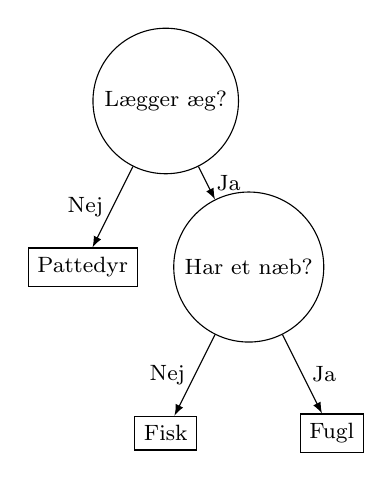
\begin{tikzpicture}
	[
	grow                    = down,
	sibling distance        = 6em,
	level distance          = 6em,
	edge from parent/.style = {draw, -latex},
	every node/.style       = {font=\footnotesize}
	]
	\node [node_] {Lægger æg?}
	child { node [leaf_] {Pattedyr}
		edge from parent node [left] {Nej} }
	child { node [node_] {Har et næb?}
		child { node [leaf_] {Fisk}
			edge from parent node [left]{Nej} }       
		child { node [leaf_] {Fugl}
			edge from parent node [right]{Ja} }
		edge from parent node [right] {Ja} };
	\end{tikzpicture}
\end{center}
Dette ser undertiden fint ud, men prøver man sætte et næbdyr ind i denne model, vil den blive klassificeret som en fugl (da den har et næb og lægger æg), selvom den egentlig er et pattedyr. Selvom vi egentlig har en model, som måske kan klassificere de fleste dyr korrekt, vil der være specielle tilfælde, hvor den skyder helt ved siden af. I dette eksempel kunne man muligvis løse problemet ved at indsamle flere egenskaber, og benytte et større træningssæt, men dette vil ikke altid være muligt, og der vil som sådan være situationer, hvor man ikke kan bygge en perfekt klassificeringsmodel.


\subsection{Beslutningstræer (Decision trees)}
Et eksempel på en klassificeringsteknik er gennem brug af beslutningstræer. Et beslutningstræ består af knuder og blade samt en rodknude. Et datapunkt kan da klassificeres ved at traversere træet startende i roden.

Hver knude består af et spørgsmål, som har en definitiv mængde svar, der kan besvares ud fra egenskaberne i et givent datapunkt. Ud fra svaret (altså datapunktets egenskaber) peger knuden videre til en ny knude eller et blad. Et blad repræsenterer den endelige kategori. I eksemplet i figur 1, kan der ses et eksempel på hvordan et \textit{decision tree} fungere, i dette eksempel antager vi, vi har fået en mængde, som indeholder enten biler, fly eller både, vi starter med at spørge om det givet datapunkt har hjul, hvis nej må det være en båd, hvis ja kan det enten være en bil eller et fly, og derfor spørger vi igen, denne gang om det givet datapunkt har vinger, hvis ja er det et fly, og hvis nej må det være en bil, på denne måde har vi sikret os at vores datapunkt er kommet i den rigtige kategori.

\begin{figure}[H]
\begin{center}
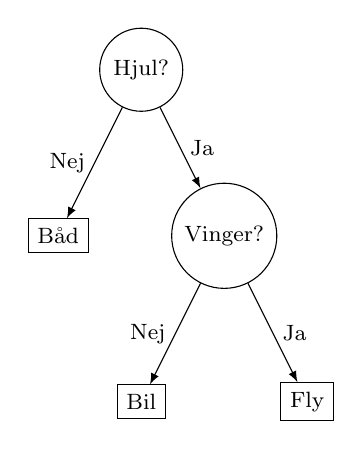
\begin{tikzpicture}
  [
    grow                    = down,
    sibling distance        = 6em,
    level distance          = 6em,
    edge from parent/.style = {draw, -latex},
    every node/.style       = {font=\footnotesize}
  ]
  \node [node_] {Hjul?}
    child { node [leaf_] {Båd}
      edge from parent node [left] {Nej} }
    child { node [node_] {Vinger?}
      child { node [leaf_] {Bil}
              edge from parent node [left]{Nej} }       
      child { node [leaf_] {Fly}
              edge from parent node [right]{Ja} }
              edge from parent node [right] {Ja} };
\end{tikzpicture}
\end{center}
\caption{\textit{Decision tree} eksempel}
\end{figure}

Et (muligvis suboptimalt) beslutningstræ kan bl.a. konstrueres fra et træningssæt med Hunts algoritme. Algoritmen starter med en mængde af alle datapunkter i træningssættet. Hvis alle punkter i mængden har samme kategori bliver denne mængde et blad i træet. Ellers stilles et spørgsmål om punkterne i mængden, og disse punkter uddeles samles i delmængder ud fra, hvordan de besvarer spørgsmålet. Spørgsmålet bliver en knude i træet, som peger på de nye delmængder, og algoritmen køres rekursivt på delmængderne.


\subsubsection{Eksempel på modeludledning}
For at illustrere brugen af decision trees vil vi her vise et eksempel på, hvordan man ud fra et todimensionelt træningssæt og testsæt kan bygge og efterteste en klassificeringsmodel. Betragt følgende træningssæt:

\begin{tabular}{c|c|c}
	X & Y & Klasse\\
	\hline
	0.8 & 0.9 & A\\
	0.6 & 0.1 & B\\
	0.2 & 0.3 & C\\
	0.1 & 0.8 & C\\
	0.4 & 0.2 & B\\
	0.4 & 0.5 & A\\
	0.03 & 0.6 & C\\
	0.5 & 0. 3 & B\\
	0.6 & 0.7 & A\\
	0.45 & 0.8 & A\\
	0.8 & 0.7 & B\\
	0.28 & 0.3 & C\\
	0.1 & 0.05 & C
\end{tabular} 

Tegner vi disse punkter ind i en graf ser det således ud:
\begin{center}
	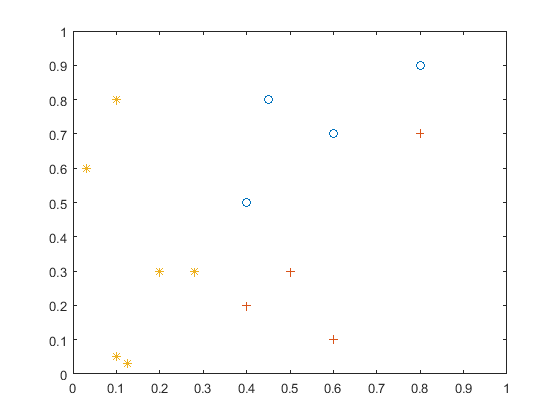
\includegraphics{decision_tree_example_plot}
\end{center}
Hvor blå cirkler er A, røde plusser er B og gule stjerner er C. Der er klare tendenser i, hvordan punkterne har fordelt sig. Ved at indtegne et par linjer kan vi tydeligt illustrere dette:
\begin{center}
	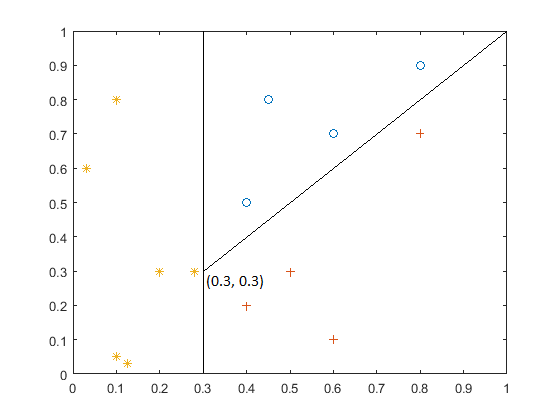
\includegraphics{decision_tree_example_plot_splitted}
\end{center}
Ud fra denne opdeling kunne det tyde på, at $f(x,y)=C$ for $x<0.3$, $f(x,y)=A$ for $0.3<x<y$ og $f(x,y)=B$ for $0.3<x$ og $y<x$. Med disse observationer kan vi bygge et beslutningstræ med Hunts algoritme.

Lad $D_t$ være hele træningssættet. Så indeholder $D_t$ punkter af alle klasser, vælger vi en (\textit{attribute test condition}) ad adskille punkterne på. For at få det mindste træ starter vi med at teste om $x<0.3$, hvilket giver også en mængde $D_{t1}=\{p\ |\ class(p)=C\}$ for ja og $D_{t2}=\{p\ |\ class(p)\neq C\}$ for $0.3<x$. Da $D_{t1}$ kun indeholder en klasse bliver dette til et $C-$blad i træet, mens vi må teste rekursivt på $D_{t2}$.

Vi tester $D_{t2}$ for egenskaben $x<y$ og får en gruppe $D_{t3}=\{p\ | class(p)=A\}$ for ja og $D_{t4}=\{p\ |\ class(p)=B\}$ for nej. Da begge disse grupper er rene (kun indeholder en punkter af en klasse) bliver disse til blade, og vi kan nu tegne vores beslutningstræ.

\begin{center}
	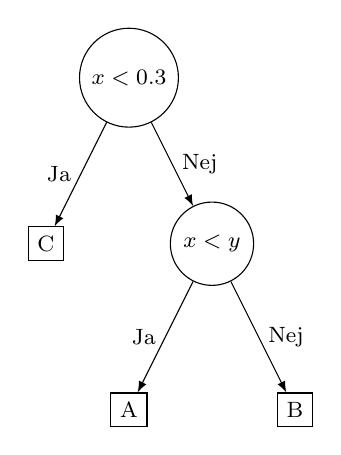
\begin{tikzpicture}
	[
	grow                    = down,
	sibling distance        = 6em,
	level distance          = 6em,
	edge from parent/.style = {draw, -latex},
	every node/.style       = {font=\footnotesize}
	]
	\node [node_] {$x<0.3$}
	child { node [leaf_] {C}
		edge from parent node [left] {Ja} }
	child { node [node_] {$x<y$}
		child { node [leaf_] {A}
			edge from parent node [left]{Ja} }       
		child { node [leaf_] {B}
			edge from parent node [right]{Nej} }
		edge from parent node [right] {Nej} };
	\end{tikzpicture}
\end{center}
Det er nu lykkedes at bygge en model, som kan opdele træningssættet korrekt. Dette er dog ingen garanti for, modellen er korrekt. Modellen er bygget ud fra nogen antagelser, som holder gennem træningssættet, men det betyder ikke, at det holder i praksis. For at undersøge modellens nøjagtighed vil vi bruge den til at klassificere testsættet nedenfor.

\begin{tabular}{c|c|c}
	X & Y & Klasse\\
	\hline
	0.2 & 0.01 & C\\
	0.28 & 0.1 & C\\
	0.1 & 0.2 & C\\
	0.4 & 0.5 & A\\
	0.5 & 0.8 & A\\
	0.9 & 0.95 & A\\
	0.5 & 0.4 & B\\
	0.8 & 0.2 & B\\
	0.6 & 0.5 & A\\
	0.7 & 0.1 & B\\
	0.5 & 0.12 & B\\
	0.12 & 0.75 & C
\end{tabular} 

Tegner vi punkterne ind i en graf med grænserne sat som før får vi følgende resultat:
\begin{center}
	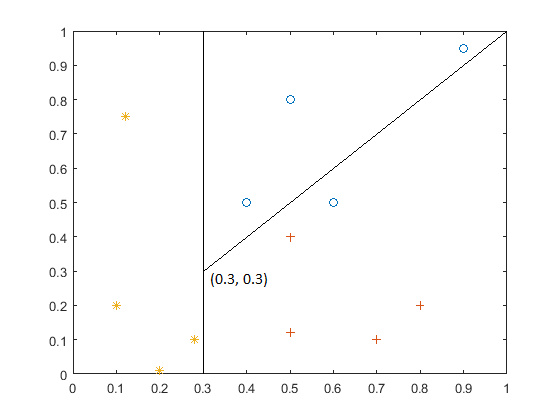
\includegraphics{decision_tree_example_plot_test}
\end{center}
Testsættet passer næsten overens, men der er et enkelt punkt som ikke overholder vores antagelse, så modellen er ikke perfekt. Helt konkret kan vi udregne en nøjagtighed baseret på vores resultat med testsættet. Ud af 12 punkter blev 11 punkter klassificeret korrekt, så vi regner os frem til en nøjagtihed $acc_M=\frac{11}{12}\approx0.92$


\section{Support Vector Machines (SVM)}

En SMV træningsalgoritme er en type klassifikationsteknik til binær klassifikation, som er specielt egnet til data af mange dimensioner. Teknikken baseres på at finde et \textit{maximal margin hyperplane}, altså et hyperplan som deler datapunkterne op i to dele svarende til deres kategori, med maksimal margin til de nærmeste punkter. Dette hyperplan betegnes som modellens \textit{decision boundary}.

Formålet med at maksimere margin er at optimere modellens generaliseringsevne, og dermed opnå bedst mulig nøjagtig når nye punkter skal klassificeres. Hvis vores decision boundary har meget lille margin, er der intuitivt ikke plads til meget forskel på dataen sammenlignet med træningssættet. Dette koncept illustreres i eksemplet nedenfor.

Betragt træningssættet af todimensionelle punkter, markeret som plusser og cirkler afhængig af deres klasse.

\begin{center}
	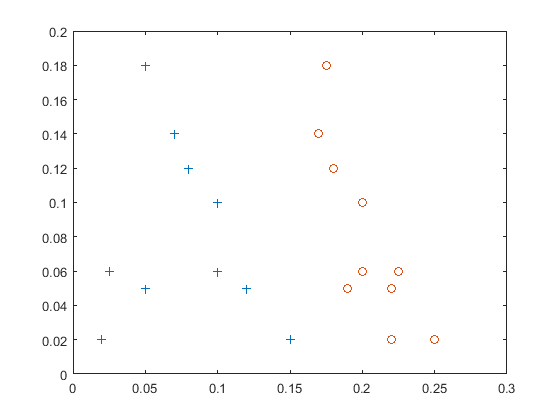
\includegraphics{maximal_margin_hyperplane_1}
\end{center}

Nedenfor er indtegnet to hyperplaner (sorte linjer) og deres margin (grå linjer), som begge deler træningssættet op uden fejl. Det er tydeligt at B2 har breddere margin end B1, og B2 er derfor objektivt den bedste løsning til problemet. Undersøger man selv dataen for en naturlig tendens i opdelingen, bliver det også tydeligt at se, at B2 følger denne tendens langt bedre end B1.

\begin{center}
	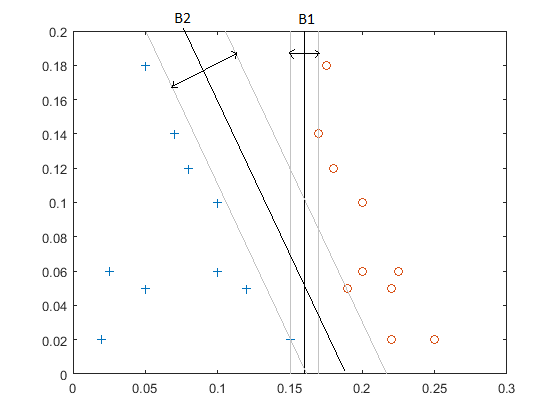
\includegraphics{maximal_margin_hyperplane_2}
\end{center}


\subsection{Linear SVM}
\subsubsection{Separable case}
\subsubsection{Non-separable case}

\subsection{Non-linear SVM}
Det er ikke altid muligt at definere en lineær opdeling af dataen. En naiv løsning på dette problem er, at transformere datapunkterne til et andet rum, hvor en lineær opdeling er mulig.

Antag at vi har en transformation $\Phi(x)$ fra det originale rum til et transformeret rum, hvor en lineær opdeling er mulig. Så kan vi genbruge vores viden fra det lineære tilfælde, og optimeringen er nogenlunde den samme. For at opnå den maksimale margin skal vi igen minimere funktionen 
$$f(w)=\frac{||w||^2}{2}$$
Under kravet at
$$y_i(w\cdot\Phi(x_i)+b)\geq 1,\text{ for }i=1,2..,N$$
Ligningen er næsten identisk med det lineære tilfælde, men vi optimerer nu med $\Phi(x_i)$ - altså $x_i$ i det transformerede rum.

Lagrange kan nu benyttes på samme måde som i det lineære tilfælde. Også her ska lvi blot benytte de transfomerede punkter.

\begin{align*}
L_D&=\sum_{i=1}^{n}\lambda_i-\frac{1}{2}\sum_{i,j}\lambda_i\lambda_j y_iy_j\Phi(x_i)\cdot\Phi(x_j)
\end{align*}

Denne optimering kræver som man kan se udregningen af prikproduktet mellem samtlige par af punkter i det transformerede rum. Da dette kan være udregningsmæssigt tungt, og kræver at man kender en transformation der passer på det enkelte problem, vil man typisk bruge en anden tilgang kaldet \textit{kernel trick}. Tilgangen bygger på et matematisk resultat, der tillader os at benytte en klasse af funktioner kaldet kernefunktioner.

For at en kernefunktion kan bruges i en ikke-lineær SVM, skal den overholde Mercers teorem. Dette medfører at der findes en transformation $\Phi$ sådan at kernefunktionen regnet på ethvert par af vektorer $u,v$ er ækvivalent til prikproduktet af $u,v$ i det transformerede rum. Altså skal det for kernefunktionen $K$ gælde at:
$$K(u,v)=\Phi(u)\cdot\Phi(v)$$

Kernefunktionen $K$ kan da erstatte prikproduktet og transformationerne i Lagrange problemet:
\begin{align*}
L_D&=\sum_{i=1}^{n}\lambda_i-\frac{1}{2}\sum_{i,j}\lambda_i\lambda_j y_iy_jK(x_i,x_j)
\end{align*}

\subsubsection{Mercers teorem}
Vi har indtil videre arbejdet med, at en kernefunktion for ethvert vektorpar $x_i,x_j$ kunne udregne prikproduktet i det transformerede rum $\Phi(x_i)\cdot\Phi(x_j)$. Lad $X=\{x_1..x_n\}$ være en mængde af vektorer. Så skal $K$ kunne udregne felterne i gram matricen $G$
\begin{align*}
G&=\left[\begin{array}{r r r}
\Phi(x_1)\cdot\Phi(x_1) & ... & \Phi(x_1)\cdot\Phi(x_n)\\\
... & ... & ...\\
\Phi(x_n)\cdot\Phi(x_1) & ... & \Phi(x_n)\cdot\Phi(x_n)
\end{array}\right]\\
\end{align*}
Da prikproduktet er symmetrisk følger det at $G$ er symmetrisk, og derfor diagonaliserbar. Altså findes der en diagonalmatrix $D$ og en invertibel matrix $P$ sådan at $P^{-1}GP=D\Leftrightarrow PDP^{-1}=G$, hvor $D$ indeholder egenværdier og $P$ indeholder tilhørende egenvektorer for $G$.

\end{document}